% main.tex, to be used with thesis.tex
% This contains the main work of your thesis.

%\bibliography{thesis}  % uses the references stored in Chapter1Radar.bib

\chapter{Data Persistence Technology for Sensor Networks: An Empirical-based
Choice for NetBEAMS}

This chapter analyzes each of the taxonomies defined in chapter
\ref{chap:taxonomies} against the requirements defined by NetBEAMS as our case
study in chapter \ref{sec:problem-requirements}, following the scope of a given
solution also defined in that chapter. The contenders were drawn from a mixed
list of technologies either related in the literature review of chapter 2 or
from the Internet.

\section{Database Systems Contenders}

This section describes the database systems contenders considered to be used
for the implementation of Data Persistence layer for NetBEAMS. As described in
the previous chapter, the selection of the technologies must be based on the
list of functional and non-functional requirements specified within the scope
of implementation defined. 

One of the primary questions related to data persistence is regarding the data
model and type of the database, such as the use of relational model or
structured models. In addition to that, and given the current time of academic
research and new trends distributed computing such as Cloud Computing and the
Internet \cite{cloud-comp-survey}, the selection of a data persistence for
sensor networks should maintain a wider spectrum of the types of database
systems. Among other intriguing questions, \cite{db-is-rdbs-dommed} reflects 
about the use of alternatives to the relational model for dynamic
environments such as data persistence for the Web. Similarly, these
trends are also related to the advances of Cloud Computing and its persistence
layer as a solution to dynamic systems \cite{cloud-comp-architectures}. For
this reason, this work also included the overview of alternative data models
for the development of an experiment that brings data persistence to NetBEAMS.

\begin{itemize}
  \item \textbf{MySQL}: an open-source relational database system that is the
  primary choice of the development of projects of different sizes. It was selected
  because of its popularity in the current community;
  \item \textbf{Oracle}: is the most popular commercial database system, having
  a campus wide academic licenses availabe;
  \item \textbf{TinyDB}\cite{tinydb}: as referred in the literature review,
  TinyDB is a database system used in many different sensor networks implementation
  \cite{sn-db-tinydb};
  \item \textbf{MongoDB}\cite{mongodb}: an open-source key-value database system
  described in the article that questions the use of the relational model
  \cite{db-is-rdbs-dommed}, as well as the Cloud Computing trends survey
  \cite{cloud-comp-architectures}.
  \item \textbf{DB2}\cite{db2}: in the search of an XML database system, DB2 is
  listed as a hybrid database system that offers both XML and relational model
  \cite{db-xml-enabled}. It was selected because NetBEAMS can represent the
  collected data in the XML format \ref{sec:dsp-message}.
\end{itemize}

The following sections analyzes the taxonomies defined in chapter 3, along with
the requirements for the Data Persistence Layer for NetBEAMS, in section 4.

\section{Analysis of the Purpose of Sensor Data}

Considering the infrastructure of NetBEAMS, as described in the previous
chapter, and the characteristics of the sensor network defined at the SF-BEAMS
site \cite{sfbeams2006}, the data characteristics are as follows:

\begin{itemize}
  \item Data is generated by sensor devices, such as the YSI sonde
  \cite{YSI-Sonde}, and manually collected by using a laptop to the network
  sink at the RTC laboratories;
  \item Upon data reception, the RTC staff index and archive the data for
  for distribution using the OPEnDAP format;
  \item Another approach for data collection of data generated by the SF-BEAMS
  is the use of NetBEAMS \cite{netbeams2009}, as described in section
  \ref{netbeams-architecture}.
\end{itemize}

As summarized in the previous section, the nature of data from NetBEAMS through
SF-BEAMS is used for the purpose of \textbf{Data Archival}.

\subsection{Technology Analysis}

As it is supposed to be, all the contenders are developed to support data
persistence and management, what is the requirement for the Data Archival
purpose of the sensor network data.

\begin{itemize}
  \item \textbf{MySQL}: Supports
  \item \textbf{Oracle}: Supports
  \item \textbf{TinyDB}: Supports
  \item \textbf{MongoDB}: Supports
  \item \textbf{DB2}: Supports
\end{itemize}

\section{Analysis of the Location of Sensor Data Taxonomy}
\label{sec:sn-data-location}

Some observations regarding the location of the collected sensor data for
NetBEAMS were described in the previous section and summarized as follows:

\begin{itemize}
  \item NetBEAMS's architecture is based on a single-hop star infrastructure 
   with a direct network sink being the RTC server \ref{sec:sn-infrastructure}.
\end{itemize}

Based in the observations also described in the previous chapter, the type used
for storing data can be either the \textbf{External Storage}. However, the use
of a \textbf{Data-Centric Storage} approach can be considered. The former is the
current approach used by the SF-BEAMS sensor network, while the latter can be
explored in the experiments.

\subsection{Advantages of the External Storage Approach}

The External Storage approach is the most common way to implement persistence
for any type of systems, including sensor networks, due to its the simplistic
data management. Furthermore, this type of setup is easier to use of
distributed systems approaches such as Replication to help preventing scaling
the system.

\subsection{Disadvantages of the External Storage Approach}

The most common problem related to a single External Data Storage is that
resources may run into data management problems such as full disk space or disk
failures.

\subsection{Advantages of the Data-Centric Approach}

The advantage of the Data-Centric approach lies on the way that data is
distributed into different locations. By using techniques of distributed
database systems, the approach improves overall performance of the use of
massive data sets since the operations of the data are directed to specific
locations. Besides, this approach helps the network managers scale the data
storage just by adding new data nodes as required.

In order to support this strategy, approaches such as data partitioning based
on the entities called Database Sharding
\cite{db-shard02}, or the partitioning based on tables
\cite{db-table-partition}. The former is a technique used in distributed
database systems that uses denormalized data models to improve scalability in
terms of data storage and data location, while the latter defines partitioning
techniques in relational databases. It is a type of database system patitioning
where de-normalized data is spread across different other hosts, or shard
\cite{db-shard01}. Different models of database sharding can be developed
\cite{db-shard-schemas}.

\begin{itemize}
  \item Vertical Partitioning: each feature of the system, usually represented
  by a table in the relational model, is placed in a different server host. For
  example, each sensor in a given network can be divided by its device type;
  \item Range Based Partitioning: after partitioning each feature on a
  different server host, different multiple shards, or similar hosts, can be
  added by using the range of a given key of the entity of a function. For
  example, all sensor types in a geographic location may contain its own shard
  based on its IP address;
  \item Key or Hash Based Partitioning: a given value for a given property of
  an instance of data that is chosen to be used in a hash function, whose
  output determines which shard to use;
  \item Directory Based Partitioning: a simple lookup service is used to
  identify which database shard to use, where the lookup table can be stored
  in a secondary area. Each approach for database sharding used be used
  together on a given function depending on the needs for performance.
\end{itemize}

For example, figure \ref{fig:database-sharding-by-region} is an example of
data storage with shards \cite{db-shard01} related the location of data, where
each shard is assumed to be placed in different server host. Since the data
model is denormalized, the organization of data is entirely placed in each of
these shards. As it is shown, the shards by location can be defined by a shard
key, as described before. The horizontal scalability is given related to
positions, while the vertical by the shards added.

\begin{figure}
  \centering
  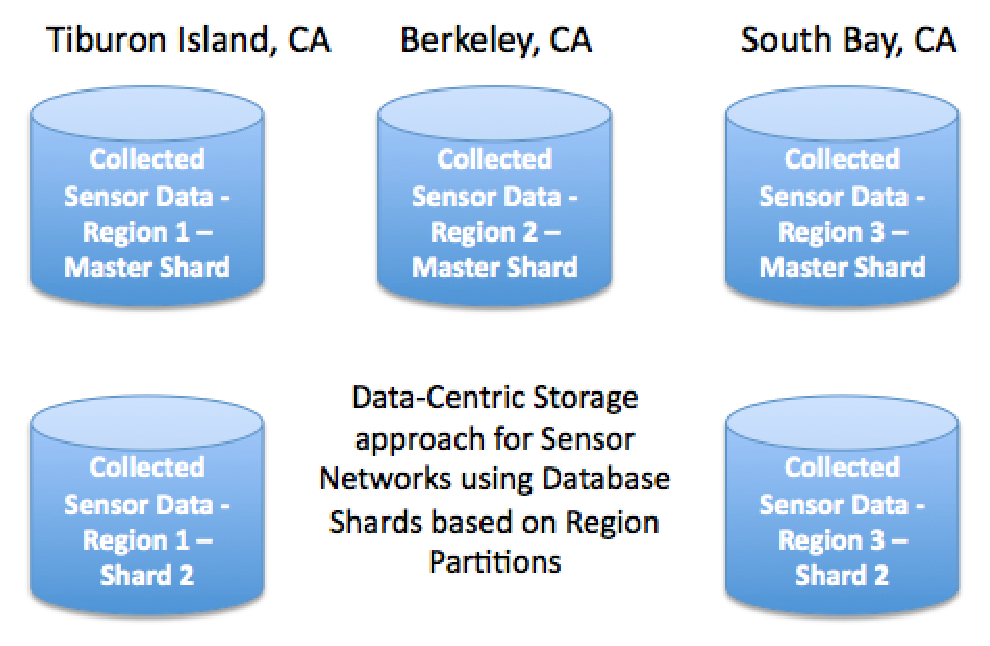
\includegraphics[scale=0.65]{../diagrams/database-sharding-by-region}
  \caption{Example of Data-Centric Storage for Sensor Networks using Database
  Sharding}
  \label{fig:database-sharding-by-region}
\end{figure}

%This data organization architecture is currently being used to manage
%structured data that scales to petabytes or more data. One example of such use
%is on BigTable \cite{bigtable}, which provides support to different Google
%products with requirements on high availability and dynamic data models and
%uses automatic sharding to its data. The BigTable project uses MapReduce
%[ds02], a programming model designed to search huge amounts of data in
%paralell.

\subsection{Disadvantages of the Data-Centric Approach}

The data partitioning is a very restricted technology, mostly available to
advanced users of distributed database systems. The main users of wireless
sensor networks do not have such expertise.

\begin{itemize}
  \item Referential integrity: any cross-shard queries can represent problems 
  since the application layer is responsible to enforce data integrity, like
  verifying constraints of foreign keys;
  \item Rebalancing Shards: If the schema model changes for the shards, the
  strategy of rebalancing must be done. For instance, when one of the shards 
  outgrows more than the others. As a consequence, the database shards must be
  rebalanced by transferring data to new locations whenever necessary. This
  technique is starting to appear as COTS implemetations such as
  \cite{mongodb}.
\end{itemize}

\subsection{Technology Analysis}

\begin{itemize}
  \item \textbf{MySQL}: Supports
  \item \textbf{Oracle}: Supports
  \item \textbf{Berkeley TinyDB}: Supports
  \item \textbf{MongoDB}: Supports
  \item \textbf{CouchDB}: Supports
  \item \textbf{DB2}: Supports
\end{itemize}

\section{Analysis of the Query Processing Mechanism Taxonomy}

As a direct result from the previous section, the use of \textbf{Centralized Query
Processing} is indicated for NetBEAMS, given the fact that NetBEAMS contains
a single network sink, and therefore, a centralized location of the data.

\subsection{Advantages of the Centralized Query Processing}

Centralized data management and query processing is simpler than in in-network.
The centralized query processing can be 

\subsection{Disadvantages of the Centralized Query Processing}

The creation of the so-called Funneling Affect, since the point-of-traffic is
concentrated in the centralized system. Any data exchange will be using the
same channel of data exchange.

\subsection{Technology Analysis}

\begin{itemize}
  \item \textbf{MySQL}: Supports
  \item \textbf{Oracle}: Supports
  \item \textbf{Berkeley TinyDB}: Supports
  \item \textbf{MongoDB}: Supports
  \item \textbf{CouchDB}: Supports
  \item \textbf{IBM DB2}: Supports
\end{itemize}

\section{Analysis of the Data Model Taxonomy}

One of the most common practices in the area of database system is to use the
relational model to persist data, although the application of the system may
not fit to solve the problem. In fact, the main users of sensor networks may
not hold any expertise in database systems or data modeling, given they come
from different science areas. Taking NetBEAMS as an example, we see a Sensor
Network managed by Marine Biologists without expertise in Data Management,
Modeling systems, and for this reason, one of the requirements of the system is
the use of schema-less approaches. The \textbf{Key-Value-Pair Data Model} or the
\textbf{Document-Oriented Data Model} seems to be the simplest choices of the
models.

\subsection{Analysis of the Schema-Dependent Models}

Considering the inception of a relational data model \cite{relational-model} and
the use of the YSI Sonde data as the main entity in the system, let figure 
\ref{fig:Relational-Model-Original} represent a prototype of the relational
model, after passing through the process of normalization
\cite{db-normalization}.

\begin{figure}
  \centering
  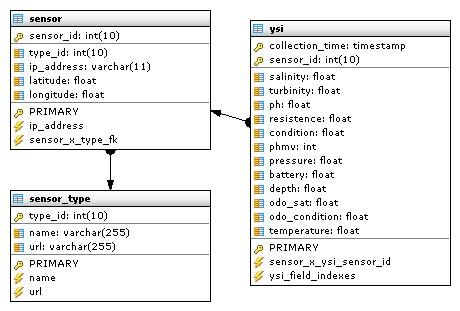
\includegraphics[scale=0.65]{../diagrams/Relational-Model-Original}
  \caption{Relational Data Model for NetBEAMS - A first prototype}
  \label{fig:Relational-Model-Original}
\end{figure}

Supposing a new type is added into the system, let the refactored
version of the relational model be depicted in figure
\ref{fig:Relational-Model-Addition-Modified}.

\begin{figure}
  \centering
  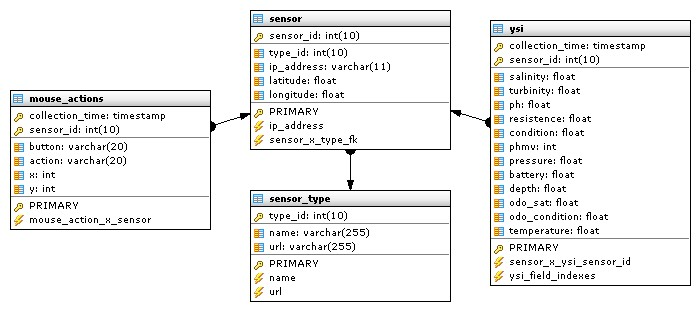
\includegraphics[scale=0.65]{../diagrams/Relational-Model-Addition-Modified}
  \caption{Relational Data Model for NetBEAMS - Modified version with new
  entity}
  \label{fig:Relational-Model-Addition-Modified}
\end{figure}

\begin{itemize}
  \item Constant data schema changes require constant database normalization
  process, changes to structure, database management, etc;
  \item Some research have shown that the Relational Model does not fit the
  nature of collected data from wired or wireless sensor networks. They usually
  does not support time-series data nor provenance.
  \item Even project aiming at updating the relational sensor database systems
  and SQL clauses have been proposed. 
\end{itemize}

Other projects have been using the XML data models. It falls into the same
category as the Relational Model, since the XML documents \cite{xml}, when in
the context of a database, must be complaint to an XML Schema \cite{xml-schema}. As shown in
section 3, this model uses XPath \cite{xml-xpath} technology for querying
documents, although some hibrid technologies may still use SQL \cite{sql} for
that matter. In this way, an instance of such schema dependent types can be
seen in figure \ref{fig:persistence-example-relational}.

\begin{figure}[!h]
  \centering
  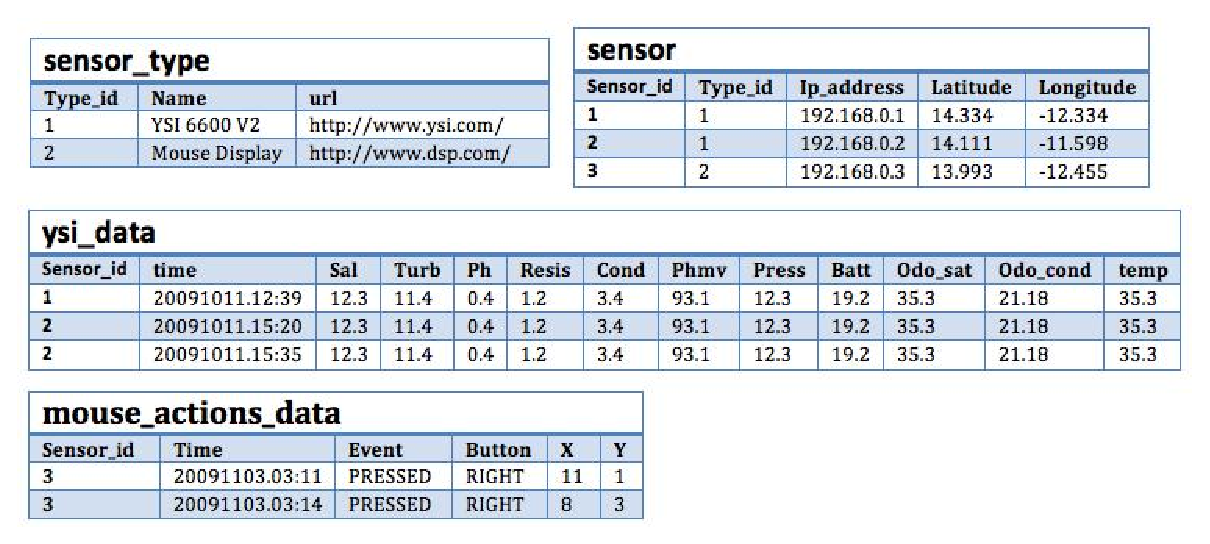
\includegraphics[scale=0.7]{../diagrams/persistence-example-relational}
  \caption{Instance of a Relational Model Database Prototype}
  \label{fig:persistence-example-relational}
\end{figure}

Although this data model have been used in different types of applications,
developers have tried to use the Relational Model to model an application that
could prevent any database change through the use of a technique that relates a
key to a value, called Key-Value data model. With the advent of Internet
applications, the need of such a model that does not need constant refactoring
led developers to propose such approach using the relational model as
documented in technical articles such as \cite{db-kvp-in-relational01} and
\cite{db-kvp-in-relational02}. Based in these articles, consider the relational
model depicted in figure \ref{fig:KVP-on-Relational-Model} as model for the
persistence data for our case study using the key-value strategy. The problem
with it is that key repetition occurs, since the nature of time-series data
requires the use of a timestamp key for each property of the sensor. Therefore,
this strategy is not well-suited to provide persistence data from collected
sensor networks.

\begin{figure}[!h]
  \centering
  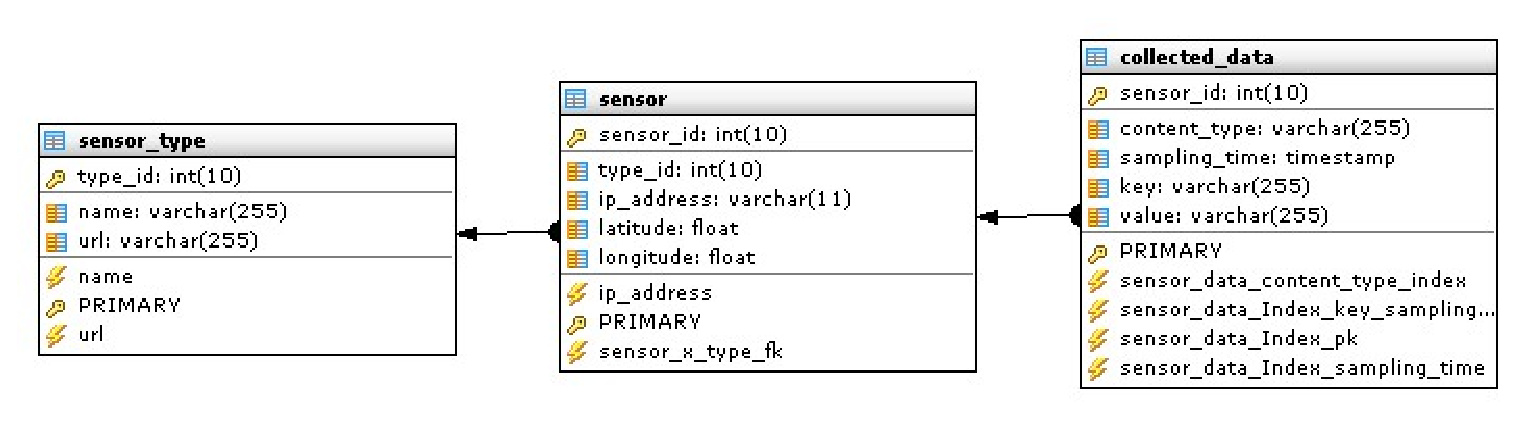
\includegraphics[scale=0.6]{../diagrams/KVP-on-Relational-Model}
  \caption{KVP Data Model implementation using Relational Model}
  \label{fig:KVP-on-Relational-Model}
\end{figure}

\begin{figure}[!h]
  \centering
  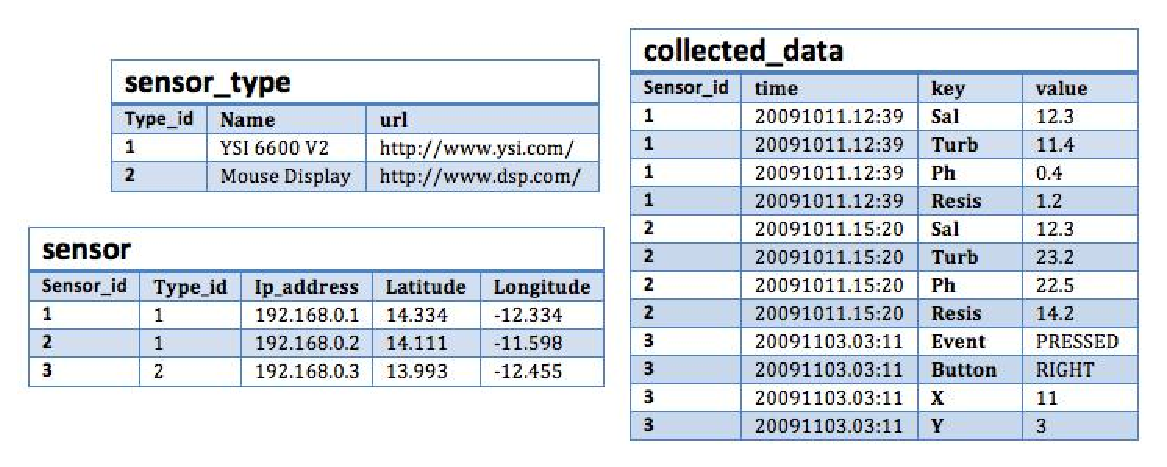
\includegraphics[scale=0.75]{../diagrams/persistence-example-relational-kvp}
  \caption{KVP over Relational Model Database Prototype}
  \label{fig:persistence-example-relational-kvp}
\end{figure}

\subsection{Analysis of the Schema-less Models}

The growth of distributed systems and the Internet have enabled the development
of powerful database servers that can be organized in the context of
infrastructure and how to represent models. An powerful up-coming approach is
the use of database systems that does not use structured language for querying
its data. One such example is called Key-Value Pair (KVP) data model
\cite{db-kvp}, which is also known as Document-Oriented, Distributed Hash
Table. Such a model has the following properties:

\begin{itemize}
  \item data is structured in collections of key-value pairs, as it is done in
  hash data structure. The definition of the key is a given property with its
  associating value;
  \item the query process is using mechanics similar to programming or
  scripting language, that is, the use of APIs in a given programming language.
\end{itemize}

There are no records of the use of this data model with Sensor Networks.
Different variants of such data model is the document-oriented data model,
where data is modeled using structured documents. However, these documents
have a dynamic structure that can be freely described without the use of a
schema validation mechanism as used in XML Schema. One example of such
approach is the use of the JSON data format \cite{json} in the implementation
of database systems which are becoming popular with the new trend called Cloud
Computing \cite{cloud-comp-architectures}. Databases implementing this
strategy is the mongoDB \cite{mongodb}.

\begin{itemize}
  \item entities from the same domains are placed into a bucket;
  \item entities have a set of attributes and relating values
  \item entities with different set of attributes may be contained in the same
  bucket, since there is no schema to govern the bucket items restriction.
\end{itemize}

For instance, all data needed for the YSI sonde data, as well as all necessary
provenance data that describes the data, depicted in section
\ref{sec:sn-provenance}, are represented by means of key-value pairs
\ref{fig:persistence-example-kvp}.

\begin{figure}[!h]
  \centering
  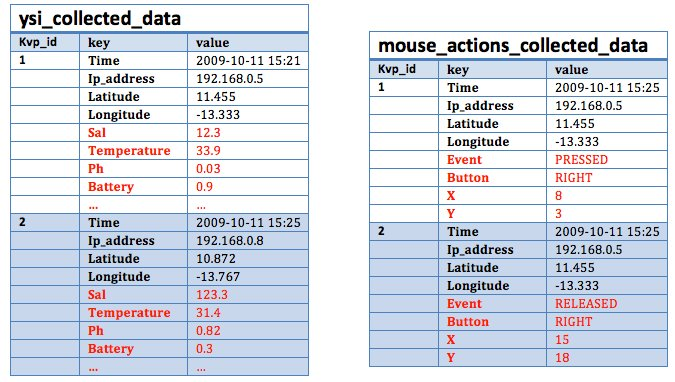
\includegraphics[scale=0.75]{../diagrams/persistence-example-kvp}
  \caption{KVP Database instance Prototype}
  \label{fig:persistence-example-kvp}
\end{figure}

\subsection{Technology Analysis}

The relational and key-value data models were compared by
\cite{db-is-rdbs-dommed} and can be summarized as follows:

\begin{table}
    \label{tab:ysi-data-distribution}
    \caption{Schema-Dependent X Schema-less Databases Compared: Properties}
    \begin{center}
    \begin{tabular}{|p{210pt}|p{210pt}|}\hline
    Schema-Dependent Databases & Schema-less Databases\\\hline
    \begin{enumerate}
      \item Real-world model by entities, classified in tables;
      \item Tables composed by columns and rows. Rows are comprised by column
      values, which have the same schema;
      \item Data Model defined in advance with a schema, which contains
      relationships and constraints to enforce data integrity;
      \item Data represents ``natural'' entities, not application specific;
      \item Data Normalization is the data structuring process to remove data
      duplication, as well as establishing data associations through table
      relationships;
      \item Data Provenance can be provided through data types such as
      ``Timestamp'' for time or float for the GPS float-based coordinates; 
    \end{enumerate} 
    & 
    \begin{enumerate}
      \item Real-world model by entities, classified in Domains;
      \item Domains are similar to tables, but like buckets that contains items
      without a pre-defined schema, what enable them to have different schemas;
      \item Items are identified by keys, as well as have a dynamic set of
      attributes attached to it, however with no schema defined;
      \item Items may represent not only the natural representation of data, but
      also include application-specific data;
      \item Since data may be repeated, no data normalization is done, so that
      integrity is done in the application layer;
      \item Data provenance can be added through the use of keys and relating
      values for the time information and location of the data.
    \end{enumerate}
    \\\hline
    \end{tabular}
    \end{center}
\end{table}

\begin{table}
    \label{tab:ysi-data-distribution}
    \caption{Schema-Dependent X Schema-less Databases: Data Access}
    \begin{center}
    \begin{tabular}{|p{210pt}|p{210pt}|}\hline
    Schema-Dependent Databases & Schema-less Databases\\\hline
    \begin{enumerate}
      \item The basic operations CRUD\footnote{Create-Retrieve-Update-Update
      database operations} data are performed using a structured language such
      as the SQL or XPath;
      \item Query languages can access data from different tables through
      joins, contains functions for aggregation and complex filter.
    \end{enumerate} 
    & 
    \begin{enumerate}
      \item The CRUD operations are performed via API\footnote{Application
      Programming Interface} through programming languages;
      \item Some technologies provide basic SQL-like syntax for filter criteria
      with some predicates like =, !=, <, > that ca be applied;
      \item The data and application integrity logic is placed in the
      application layer.
    \end{enumerate}
    \\\hline
    \end{tabular}
    \end{center}
\end{table}

\begin{table}
    \label{tab:ysi-data-distribution}
    \caption{Schema-Dependent X Schema-less Databases: Application Interface}
    \begin{center}
    \begin{tabular}{|p{210pt}|p{210pt}|}\hline
    Schema-Dependent Databases & Schema-less Databases\\\hline
    \begin{enumerate}
      \item Have their own specific API or through ODBC\footnote{Open Database
      Connectivity};
      \item Data is stored in a format that represents its natural structure,
      and for this reason, in a single or distributed fashion.
    \end{enumerate} 
    & 
    \begin{enumerate}
      \item Systems tend to provide SOAP/REST \cite{http-rest};
      \item \cite{db-is-rdbs-dommed} claims that data is stored in a more
      effective way, requiring only code plumbing for the relational code;
    \end{enumerate}
    \\\hline
    \end{tabular}
    \end{center}
\end{table}

\begin{itemize}
  \item MySQL: NO SUPPORT
  \item Oracle: NO SUPPORT
  \item Berkeley TinyDB: NO SUPPORT
  \item \textbf{MongoDB}: Supports Both
  \item IBM DB2: NO SUPPORT
\end{itemize}

\section{Analysis of the Database System Organization Taxonomy}

Sensor Network data can be saved in either Centralized or Distributed Systems.
While Centralized Database Systems are easier to manage, it may
face challenges regarding its data. In order to implement a Data-Centric
solution, a distribute database system must be in place in order to manage
the different data by a single node.

\subsection{Advantages of Database Partitioning and Sharding}

\begin{itemize}
  \item Data-Centric queries and data use;
  \item Solves bottleneck problems related to reads/writes;
  \item Decrease the funneling effect by directing queries to given data
  partition;
\end{itemize}

\subsection{Disadvantages of Database Partitioning and Sharding}

\begin{itemize}
  \item Very advanced topics in Database System;
  \item May be easy of use, depending on the application.
\end{itemize}

\subsection{Technology Analysis}

\begin{itemize}
  \item \textbf{MySQL}: Supports
  \item \textbf{Oracle}: Supports
  \item \textbf{Berkeley TinyDB}: NO Supports
  \item \textbf{MongoDB}: Supports
  \item \textbf{CouchDB}: Supports
  \item \textbf{IBM DB2}: Supports
\end{itemize}

\section{Other Non-Functional Analysis}

\begin{itemize}
  \item Given the fact of the nature of the project, the technology to be used
  must be \textbf{open-source} \cite{open-source}, that is, no costs involved
  in the adoption of such technology;
  \item A solution for persisting collected sensor data must be not only limited
  to a technology that provides data access, such as SQL, but also by other
  \textbf{data access mechanisms} such as through \textbf{native APIs}. The
  reason is that part of the sensor network data does not have skills in
  database models, but may have skills with programming languages;
  \item Supports hot backup without service interruption.
\end{itemize}

\subsection{Technology Analysis}

Most of the technologies listed provides access to the data sets through the
use of drivers in different programming and scripting languages such as Java,
Python, Perl, etc.

\begin{itemize}
  \item \textbf{MySQL}: Supports
  \item \textbf{Oracle}: Supports, Not Open-Source
  \item \textbf{Berkeley TinyDB}: Supports, Open-Source
  \item \textbf{MongoDB}: Supports
  \item \textbf{CouchDB}: Supports
  \item \textbf{IBM DB2}: Supports, Open-Source
\end{itemize}

\section{Global Analysis Results and Technology Selection}

Each of the databases were scored according to its support to the different
types of taxonomies, and randomly selected by using the literature review's
list, as well as the Internet.

\begin{table}
    \label{tab:ysi-data-distribution}
    \caption{Amount of data produced by the RTC's YSI sondes}
        \begin{center}
        \begin{tabular}{|c|c|c|c|c|c|c|}\hline 
        \textbf{Database} & \textbf{MySQL} & \textbf{Oracle} &
        \textbf{TinyDB} & \textbf{MongoDB} & \textbf{IBM DB2}\\\hline 
        Centralized Query & + & + & + & + & + \\\hline 
        Distributed System & ++ & ++ & - & ++ & +\\\hline 
        Schema-less & - & - & - & + & +\\\hline 
        Provenance Support & + & + & + & + & +\\\hline 
        NO-SQL Query & - & - & - & + & +\\\hline 
        Data Partition & + & + & - & + & +\\\hline 
        Hot Backup & + & + & - & - & +\\\hline 
        Export Capability & + & + & - & + & -\\\hline 
        Programming Lang. & + & + & + & + & +\\\hline
        Script Lang. & + & + & - & + & +\\\hline
        Open-Source & + & - & + & + & -\\\hline
        \end{tabular}
        \end{center}
\end{table}
